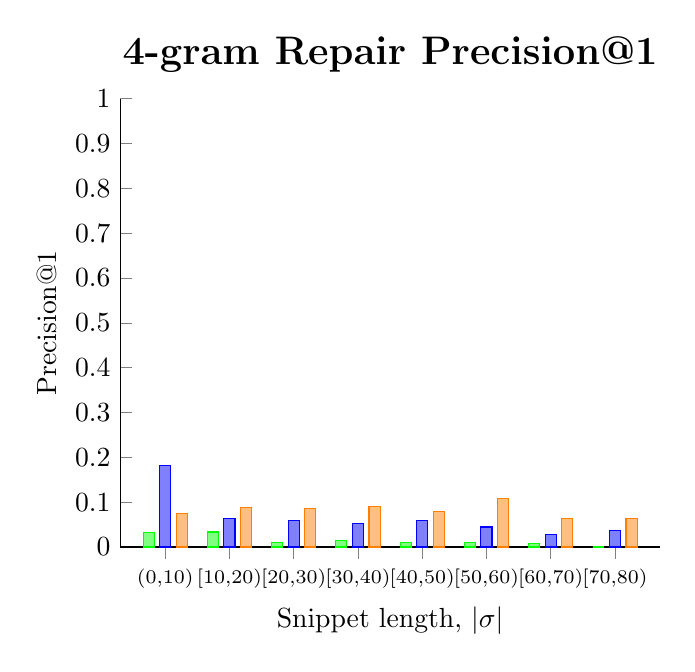
\begin{tikzpicture}
  \begin{axis}[
  xlabel={Snippet length, $|\sigma|$},
  ylabel={Precision@1},
  title={\Large\textbf{4-gram Repair Precision@1}},
  ybar,
  axis lines*=left,
  xtick={0, 10, 20, 30, 40, 50, 60, 70},
  ytick={0, 0.1, 0.2, 0.3, 0.4, 0.5, 0.6, 0.7, 0.8, 0.9, 1.0},
  xticklabels={{(}0{,}10{)}, {[}10{,}20{)}, {[}20{,}30{)}, {[}30{,}40{)}, {[}40{,}50{)}, {[}50{,}60{)}, {[}60{,}70{)}, {[}70{,}80{)}},
  x tick label style={font=\scriptsize},
  ymax=1.0,
  ymin=0.0,
  bar width=4pt,
  ]
  \addplot[green, fill=green!50] coordinates { (0, 0.03289473684210526) (10, 0.033444816053511704) (20, 0.010344827586206896) (30, 0.013793103448275862) (40, 0.010380622837370242) (50, 0.010416666666666666) (60, 0.008333333333333333) (70, 0.0) };
  \addplot[blue, fill=blue!50] coordinates { (0, 0.18095238095238095) (10, 0.06397306397306397) (20, 0.058823529411764705) (30, 0.05190311418685121) (40, 0.05821917808219178) (50, 0.04455445544554455) (60, 0.027210884353741496) (70, 0.03636363636363636) };
  \addplot[orange, fill=orange!50] coordinates { (0, 0.07407407407407407) (10, 0.08904109589041095) (20, 0.08666666666666667) (30, 0.09090909090909091) (40, 0.07894736842105263) (50, 0.10833333333333334) (60, 0.06315789473684211) (70, 0.06349206349206349) };
  \end{axis}
\end{tikzpicture}